The missing transverse energy is used to reject background events
where there is no natural source of missing energy, like in Drell-Yan and
QCD events. The residual background in the signal region is mainly from events with 
fake \met due to mismeasurement in lepton $\pt$, mismeasurement of the 
additional jets in the event, or from detector noise. 
We use the particle flow based \met variable in this analysis. 
The selection requirement on $\text{pfMET}$ at the $\ZZ$ pre-selection level is $\text{pfMET}>50~\GeV$. 

%In the presence of high multiple-interactions (pile-up), the instrumental \met\ tail in 
%$\dyll$ events increases significantly.  To improve the signal over background performance of \met\ selections 
%in the presence of pile-up, we make use of the ``trk-MET''~\cite{trkMET}, constructed from 
%charged particles consistent with originating from the primary vertex. This variable is introduced and successfully 
%commissioned in the $\hww$ analysis~\cite{HWW2011AN}, defined as:
%%%%%%%%%%%%%%%%%%%%%%%%%%%%%%%%%%%%%%%%%%%
%\begin{equation}
%\text{trk-MET} \equiv -\overrightarrow{p_T}(l_1) - \overrightarrow{p_T}(l_2) - \sum_i{\overrightarrow{p_T}(i)}, \\
%\label{eq:trkmet}
%\end{equation}
%%%%%%%%%%%%%%%%%%%%%%%%%%%%%%%%%%%%%%%%%%%

%where $\overrightarrow{p_T}(l_1)$ and $\overrightarrow{p_T}(l_2)$ are the transverse momentum vectors of the two 
%leptons passing the lepton selections described in Sec.~\ref{sec:sel_muons} and Sec.~\ref{sec:sel_electrons}, 
%and $\overrightarrow{p_T}(i)$ represent the tranverse momentum vectors of the charged PFCandidates satisfying the following requirements:
%%%%%%%%%%%%%%%%%%%%%%%%%%%
%\begin{itemize}
%\item the track matched to PFCandidate has $\Delta z < 0.1$~cm with respect to the signal primary vertex;
%\item the track has $\Delta R > 0.1$ with respect to both leptons, to avoid double-counting of the leptons.
%\end{itemize}
%%%%%%%%%%%%%%%%%%%%%%%%%%

%These two variations of \met\ are weakly-correlated in $\dyll$ background, and 
%strongly correlated for the signal processes with geninue $\met$. %, as shown in Figure~\ref{fig:met_scatter}. 
%Therefore the signal over background ratio is improved if we select the events 
%based on the mininum of these two projected $\met$ values, $\text{min-MET} \equiv min(\text{trk-MET}, \text{PFMET})$. 
%In addition, the background selection efficiency dependendence on the 
%number of primary vertices is largely reduced as well using min-MET~\cite{HWW2011AN}. 
%The selection requirement on $\text{min-MET}$ at the $\ZZ$ pre-selection level is min-MET $>50~\GeV$. 
%%%%%%%%%%%%%%%%%%%%%%%%%%%%%%%%%%%%%%%%%%%
%\begin{figure}[hbt]
%\begin{center}
%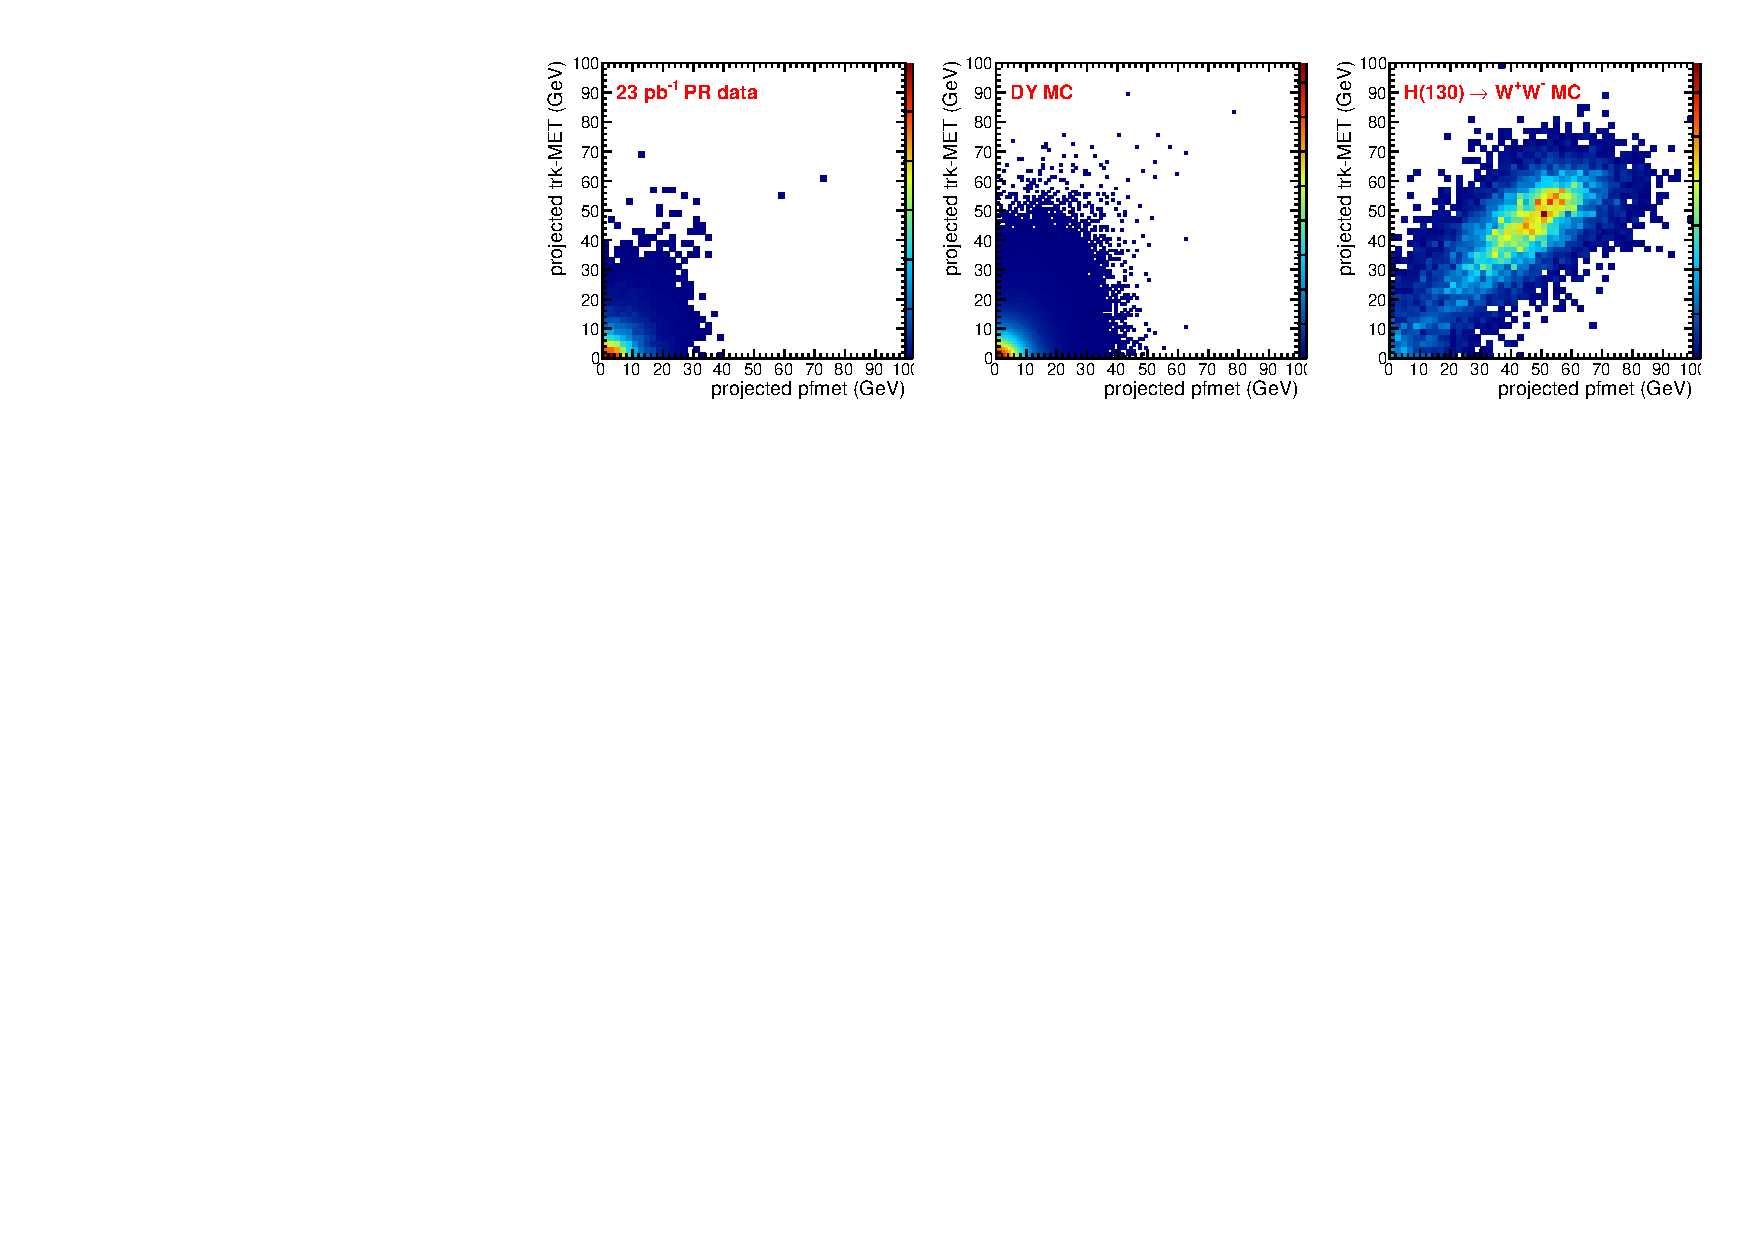
\includegraphics[width=1\linewidth]{figures/met_scatter.pdf} 
%\caption{\label{fig:met_scatter}\protect Distributions of trk-MET vs. pfmet in data (left), 
%$\dyll$ MC (center) and Higgs $\rightarrow$ WW MC (right).}
%\end{center}
%\end{figure}
%%%%%%%%%%%%%%%%%%%%%%%%%%%%%%%%%%%%%%%%%%%




%The selection efficiencies for the signal ($\hzz$ at $m_{H}=200$ GeV) and background ($\dyll$) 
%events are shown in Figure~\ref{fig:met_eff} as a function of $\met$ requirements. 
%Using min-MET we see that the signal selection efficiency improves while the background selection efficiency reduces significantly 
%compared to the values obtained using projected PFMet. 
